%<TpX v="&#9;" TeXFormat="&#9;&#9;&#9;&#9;" PdfTeXFormat="&#9;&#9;&#9;&#9;" ArrowsSize="&#9;&#9;&#9;" StarsSize="&#9;" DefaultFontHeight="&#9;" DefaultSymbolSize="&#9;&#9;" ApproximationPrecision="&#9;&#9;&#9;&#9;" PicScale="&#9;" Border="&#9;" BitmapRes="&#9;&#9;&#9;&#9;&#9;" HatchingStep="&#9;" DottedSize="&#9;&#9;&#9;" DashSize="&#9;" LineWidth="&#9;&#9;&#9;" TeXFigure="&#9;&#9;&#9;&#9;">
%  <circle x="&#9;&#9;" y="&#9;&#9;" d="&#9;&#9;&#9;&#9;&#9;&#9;&#9;"/>
%  <star x="&#9;&#9;" y="&#9;&#9;" d="&#9;&#9;&#9;"/>
%  <star x="&#9;&#9;" y="&#9;&#9;" d="&#9;&#9;&#9;"/>
%  <star x="&#9;&#9;" y="&#9;&#9;" d="&#9;&#9;&#9;"/>
%  <star x="&#9;&#9;" y="&#9;&#9;" d="&#9;&#9;&#9;"/>
%  <star x="&#9;&#9;" y="&#9;&#9;" d="&#9;&#9;&#9;"/>
%  <text x="&#9;&#9;&#9;&#9;" y="&#9;&#9;&#9;&#9;" t="&#9;&#9;&#9;&#9;&#9;&#9;&#9;&#9;" h="&#9;"/>
%  <text x="&#9;&#9;" y="&#9;&#9;" t="&#9;&#9;&#9;&#9;&#9;&#9;&#9;" h="&#9;"/>
%  <star x="&#9;&#9;" y="&#9;&#9;" d="&#9;&#9;&#9;"/>
%  <star x="&#9;&#9;" y="&#9;&#9;" d="&#9;&#9;&#9;"/>
%  <star x="&#9;&#9;" y="&#9;&#9;" d="&#9;&#9;&#9;"/>
%  <star x="&#9;&#9;" y="&#9;&#9;" d="&#9;&#9;&#9;"/>
%  <star x="&#9;&#9;" y="&#9;&#9;" d="&#9;&#9;&#9;"/>
%  <star x="&#9;&#9;" y="&#9;&#9;" d="&#9;&#9;&#9;"/>
%  <star x="&#9;&#9;" y="&#9;&#9;" d="&#9;&#9;&#9;"/>
%  <text x="&#9;&#9;" y="&#9;&#9;" t="&#9;&#9;&#9;&#9;&#9;&#9;&#9;&#9;" h="&#9;"/>
%  <star x="&#9;&#9;&#9;&#9;" y="&#9;&#9;" d="&#9;&#9;&#9;"/>
%  <star x="&#9;&#9;&#9;&#9;" y="&#9;&#9;" d="&#9;&#9;&#9;"/>
%  <star x="&#9;&#9;&#9;&#9;" y="&#9;&#9;" d="&#9;&#9;&#9;"/>
%  <star x="&#9;&#9;&#9;&#9;" y="&#9;&#9;" d="&#9;&#9;&#9;"/>
%  <star x="&#9;&#9;&#9;&#9;" y="&#9;&#9;" d="&#9;&#9;&#9;"/>
%  <star x="&#9;&#9;&#9;&#9;" y="&#9;&#9;" d="&#9;&#9;&#9;"/>
%  <star x="&#9;&#9;&#9;&#9;&#9;" y="&#9;&#9;" d="&#9;&#9;&#9;"/>
%  <star x="&#9;&#9;&#9;&#9;&#9;" y="&#9;&#9;" d="&#9;&#9;&#9;"/>
%  <star x="&#9;&#9;&#9;&#9;&#9;" y="&#9;&#9;" d="&#9;&#9;&#9;"/>
%  <star x="&#9;&#9;" y="&#9;&#9;" d="&#9;&#9;&#9;"/>
%  <star x="&#9;&#9;&#9;&#9;" y="&#9;&#9;&#9;&#9;" d="&#9;&#9;&#9;"/>
%  <line x1="&#9;&#9;" y1="&#9;&#9;" x2="&#9;&#9;" y2="&#9;&#9;&#9;" arr2="&#9;&#9;&#9;"/>
%  <line x1="&#9;&#9;" y1="&#9;&#9;" x2="&#9;&#9;&#9;" y2="&#9;&#9;" arr2="&#9;&#9;&#9;"/>
%  <text x="&#9;&#9;" y="&#9;&#9;&#9;&#9;&#9;" t="&#9;&#9;" h="&#9;"/>
%  <text x="&#9;&#9;&#9;" y="&#9;&#9;&#9;&#9;" t="&#9;&#9;" h="&#9;"/>
%  <star x="&#9;&#9;&#9;&#9;" y="&#9;&#9;&#9;&#9;" d="&#9;&#9;&#9;"/>
%  <star x="&#9;&#9;&#9;&#9;" y="&#9;&#9;&#9;&#9;" d="&#9;&#9;&#9;"/>
%</TpX>
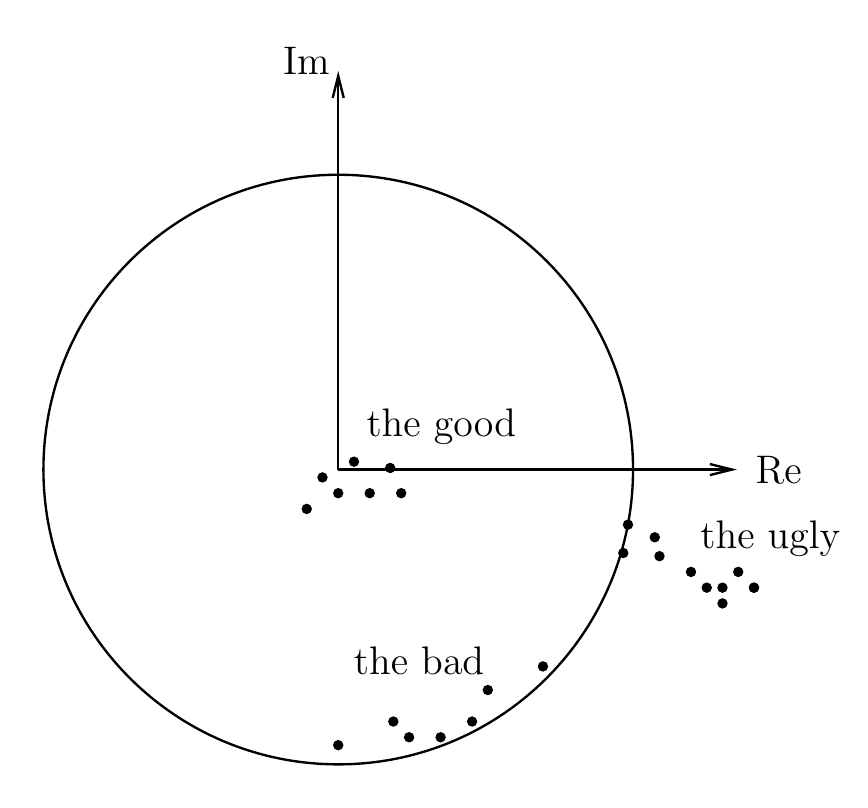
\begin{tikzpicture}[x=1.00mm, y=1.00mm, inner xsep=0pt, inner ysep=0pt, outer xsep=0pt, outer ysep=0pt]
\path[line width=0mm] (10.56,20.56) rectangle +(94.74,95.56);
\definecolor{L}{rgb}{0,0,0}
\path[line width=0.30mm, draw=L] (50.00,60.00) circle (37.44mm);
\definecolor{F}{rgb}{0,0,0}
\path[line width=0.30mm, draw=L, fill=F] (76.00,35.00) circle (0.50mm);
\path[line width=0.30mm, draw=L, fill=F] (50.00,25.00) circle (0.50mm);
\path[line width=0.30mm, draw=L, fill=F] (63.00,26.00) circle (0.50mm);
\path[line width=0.30mm, draw=L, fill=F] (50.00,57.00) circle (0.50mm);
\path[line width=0.30mm, draw=L, fill=F] (52.00,61.00) circle (0.50mm);
\draw(53.60,64.20) node[anchor=base west]{\fontsize{14.23}{17.07}\selectfont the good};
\draw(52.00,34.00) node[anchor=base west]{\fontsize{14.23}{17.07}\selectfont the bad};
\path[line width=0.30mm, draw=L, fill=F] (48.00,59.00) circle (0.50mm);
\path[line width=0.30mm, draw=L, fill=F] (46.00,55.00) circle (0.50mm);
\path[line width=0.30mm, draw=L, fill=F] (54.00,57.00) circle (0.50mm);
\path[line width=0.30mm, draw=L, fill=F] (57.00,28.00) circle (0.50mm);
\path[line width=0.30mm, draw=L, fill=F] (67.00,28.00) circle (0.50mm);
\path[line width=0.30mm, draw=L, fill=F] (69.00,32.00) circle (0.50mm);
\path[line width=0.30mm, draw=L, fill=F] (59.00,26.00) circle (0.50mm);
\draw(96.00,50.00) node[anchor=base west]{\fontsize{14.23}{17.07}\selectfont the ugly};
\path[line width=0.30mm, draw=L, fill=F] (86.80,53.00) circle (0.50mm);
\path[line width=0.30mm, draw=L, fill=F] (94.80,47.00) circle (0.50mm);
\path[line width=0.30mm, draw=L, fill=F] (96.80,45.00) circle (0.50mm);
\path[line width=0.30mm, draw=L, fill=F] (98.80,45.00) circle (0.50mm);
\path[line width=0.30mm, draw=L, fill=F] (90.80,49.00) circle (0.50mm);
\path[line width=0.30mm, draw=L, fill=F] (98.80,43.00) circle (0.50mm);
\path[line width=0.30mm, draw=L, fill=F] (100.80,47.00) circle (0.50mm);
\path[line width=0.30mm, draw=L, fill=F] (102.80,45.00) circle (0.50mm);
\path[line width=0.30mm, draw=L, fill=F] (102.80,45.00) circle (0.50mm);
\path[line width=0.30mm, draw=L, fill=F] (58.00,57.00) circle (0.50mm);
\path[line width=0.30mm, draw=L, fill=F] (56.60,60.20) circle (0.50mm);
\path[line width=0.30mm, draw=L] (50.00,60.00) -- (50.00,110.00);
\path[line width=0.30mm, draw=L, fill=F] (50.00,110.00) -- (49.30,107.20) -- (50.00,110.00) -- (50.70,107.20) -- (50.00,110.00) -- cycle;
\path[line width=0.30mm, draw=L] (50.00,60.00) -- (100.00,60.00);
\path[line width=0.30mm, draw=L, fill=F] (100.00,60.00) -- (97.20,60.70) -- (100.00,60.00) -- (97.20,59.30) -- (100.00,60.00) -- cycle;
\draw(43.00,110.20) node[anchor=base west]{\fontsize{14.23}{17.07}\selectfont Im};
\draw(103.00,58.20) node[anchor=base west]{\fontsize{14.23}{17.07}\selectfont Re};
\path[line width=0.30mm, draw=L, fill=F] (86.20,49.40) circle (0.50mm);
\path[line width=0.30mm, draw=L, fill=F] (90.20,51.40) circle (0.50mm);
\end{tikzpicture}%
